\chapter{Methodology}
\label{chapter:Methods}

In this section, the pipeline followed in this study is explained. Moreover, Fig. \ref{fig:pipeline} depicts the process, starting from the gathering of the data (preprocessing phase) and finishing with the comparison of GWAS and the obtained results (analytic phase).

\begin{figure}[h]
    \centerline{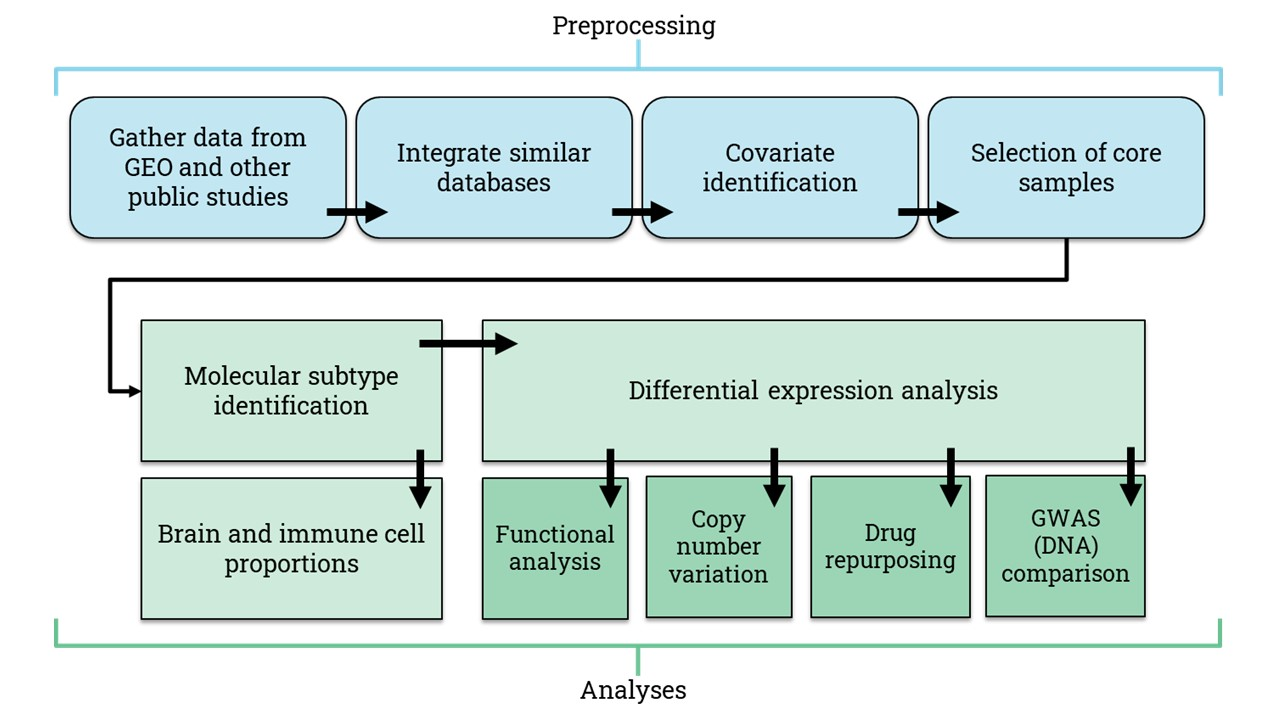
\includegraphics[width = 15cm]{Figures/pipeline.jpg}}
\caption{Pipeline employed in this study.}
\label{fig:pipeline}
\end{figure}

\section{Preprocessing}
\subsection{Downloading}

As mentioned in Fig. \ref{fig:pipeline}, the first step of the preprocessing phase is to download the required data. In order to complete this step, a profuse search in GEO Datasets platform was carried out, filtering by "expression profiling by high throughput sequencing", "human", and "AD", "PD" or "HD". At the end of the search, public RNA-seq expression data was also looked for in other databases and published papers; this search was conducted until September 1\textsuperscript{st}, 2020. After the selection of the data was concluded, the downloading step was performed using \textit{GEOquery} package; the selected datasets are presented in Table \ref{tab:samples}. Specifically, the \verb|getGEOSuppFiles| function was used since the expression data were placed as supplementary file for each sample. Likewise, the clinical information stored in the platform was downloaded by the \verb|getGEO| and \verb|pData| functions of the same R package. However, some of the clinical information was incomplete or missing in the series stored in GEO Datasets, hence a manual collection was done by searching for this information on the respective research paper. Regardless of the manual collection, clinical information of GSE64810 and GSE129473 datasets was not found. On the other hand, the data collected from other public sources (BMC and AIBS datasets in Table \ref{tab:samples}) were downloaded as a compressed folder from the online supplementary material.

\begin{table}[!ht]
\centering
\small
\caption{Metadata of the samples employed in this study.}
\label{tab:samples}
\begin{tabular}{llcccccc}
\textbf{} &
  \textbf{} &
  \multicolumn{1}{l}{\textbf{}} &
  \multicolumn{2}{c}{\textbf{Female}} &
  \multicolumn{2}{c}{\textbf{Male}} &
  \multicolumn{1}{l}{\textbf{}} \\ \cline{4-7}
\textbf{Database} &
  \textbf{Tissue} &
  \multicolumn{1}{l}{\textbf{Disease}} &
  \multicolumn{1}{l}{\textbf{Control}} &
  \multicolumn{1}{l}{\textbf{Case}} &
  \multicolumn{1}{l}{\textbf{Control}} &
  \multicolumn{1}{l}{\textbf{Case}} &
  \multicolumn{1}{l}{\textbf{Total}} \\ \hline
GSE51799                                           & Peripheral   blood       & HD & 18 & 49 & 15 & 42  & 124                  \\
GSE61405                                           & Peripheral   blood       & HD & 6  & 4  & 2  & 7   & 19                   \\
\textbf{GSE64810}                                           & Prefrontal   cortex      & HD &  & 20 & 49 &              & 69 \\
\textbf{GSE129473}                                          & Prefrontal   cortex      & HD &  & 11  & 5  &             & 16  \\
GSE68719                                           & Prefrontal   cortex      & PD & 0  & 0  & 44 & 29  & 73                   \\
GSE135036                                          & Prefrontal   cortex      & PD & 1  & 3  & 11 & 21  & 36                   \\
BMC \cite{BMC-PD}     & Prefrontal   cortex      & PD & 11 & 12 & 11 & 15  & 49                   \\
GSE67333	& Hippocampus &	AD &	2 &	3 &	2 &	1 &	8 \\
GSE104704                                          & Temporal   lobe          & AD & 1  & 1  & 9  & 11  & 22                   \\
GSE125050                                          & Superior   frontal gyrus & AD & 17 & 17 & 40 & 19  & 93                   \\
GSE125583                                          & Fusiform   gyrus         & AD & 33 & 97 & 37 & 122 & 289                  \\
GSE144254                                          & Inferior   parietal lobe & AD & 0  & 22 & 0  & 20  & 42                   \\
AIBS \cite{AIBS} & Frontal white matter   & AD & 18 & 16 & 29 & 22  & 85\\
                                                   & Hippocampus              & AD & 20 & 18 & 30 & 18  & 86                   \\
                                                   & Parietal   cortex        & AD & 18 & 16 & 28 & 21  & 83                   \\
                                                   & Temporal   cortex        & AD & 19 & 18 & 31 & 23  & 91                   \\ \cline{8-8}  
  &   &   &   &   &   &   &   1185\\                                   
\hline
\end{tabular}
\footnotesize Databases in bold does not contain clinical information other than the condition.

\end{table}

\subsection{Integration of common databases} \label{integration-method}

As it can be seen in Table \ref{tab:samples}, there are some datasets which come from the same tissue, or tissues in close proximity (Fig. \ref{fig:brain}), and have a common diagnosis; these datasets were integrated into one, named from now after, integrated datasets (see Table \ref{tab:integrated-tissue}). Moreover, GSE125583 dataset was large enough ($n=289$) to be analyzed by its own, called from now on Fusiform AD (Fus-AD) dataset. In order to integrate the datasets, the shared genes between similar datasets were identified and then, the exclusive genes were filtered. Subsequently, the integrated datasets were normalized using \verb|normalize.quantiles| function of the \textit{preprocessCore} R package. Quantile normalization is a powerful method which makes two or more distributions statistically identical; it is commonly used to equalize the distributions of different microarray's probe intensities \cite{bolstad}.

\begin{figure}[ht]
    \centerline{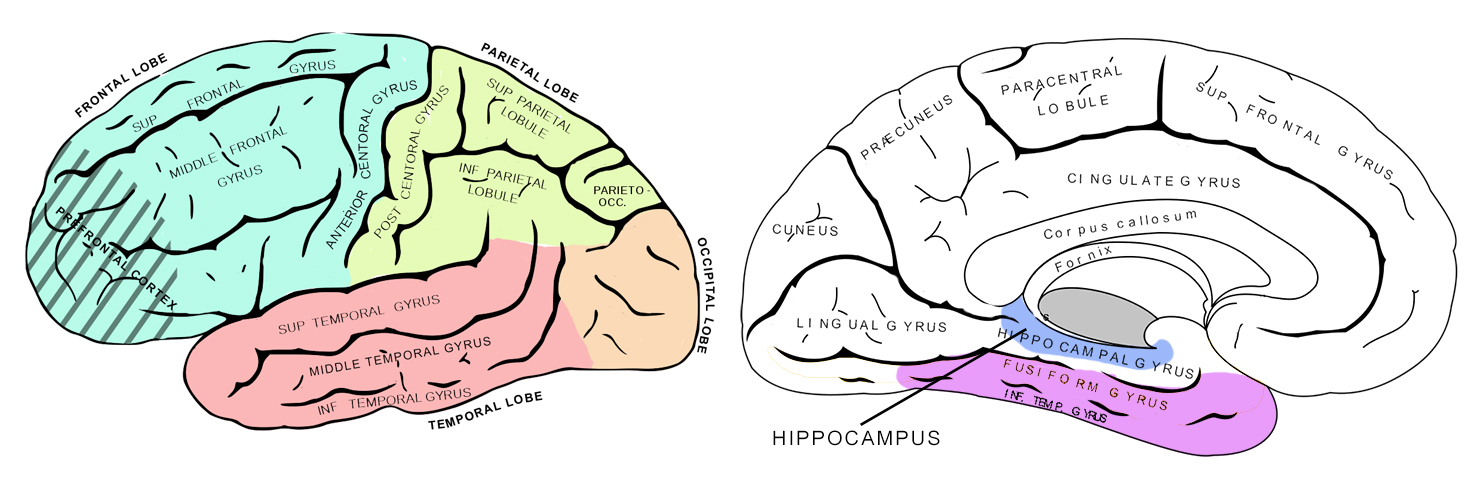
\includegraphics[width = 15cm]{Figures/brain.jpg}}
\caption{Diagram of the brain's lateral (left) and medial surface (right).}
\label{fig:brain}
\end{figure}

\begin{table}[ht]
\centering
\caption{Tissues and databases of the integrated datasets.}
\label{tab:integrated-tissue}
\begin{tabular}{lll}
\hline
\multicolumn{1}{c}{\textbf{Integrated dataset}} & \multicolumn{1}{c}{\textbf{Databases}} & \multicolumn{1}{c}{\textbf{Tissues}} \\ \hline
Prefrontal cortex PD & GSE68719     & Prefrontal Cortex      \\
                     & GSE135036    & Prefrontal Cortex      \\
                     & BMC & Prefrontal Cortex      \\
Prefrontal cortex HD & GSE64810     & Prefrontal Cortex      \\
                     & GSE129473    & Prefrontal Cortex      \\
Parietal AD          & GSE144254    & Inferior parietal lobe \\
                     & AIBS         & Parietal cortex        \\
Blood HD             & GSE51799     & Peripheral blood       \\
                     & GSE61405     & Peripheral blood       \\
Temporal AD          & GSE104704    & Temporal lobe          \\
                     & AIBS         & Temporal cortex        \\
Hippocampus AD       & GSE67333     & Hippocampus            \\
                     & AIBS         & Hippocampus            \\
Frontal AD           & GSE125050    & Superior frontal gyrus \\
                     & AIBS         & Frontal white matter   \\ \hline
\end{tabular}
\end{table}

Afterwards, the integrated datasets were adjusted to remove the batch effect. For this, principal component analysis (PCA) plots were generated using the 2,000 genes with higher median absolute deviation (MAD) before batch correction in order to identify this effect. Then, \verb|ComBat| of \textit{sva} package was leverage to proceed with the batch correction. This function needs a model and a data matrix as input; here, the model was defined as a linear model without intercept of only the batch data. Likewise, parametric adjustments were selected to be used (par.prior argument). Finally, a second set of PCA plots were generated using the 2,000 genes with higher MAD after the batch correction.

\subsection{Covariate identification} \label{cov-method}

After examining the group formation of the integrated and Fus-AD datasets in the MAD PCA plots, it was suggested than an important covariate was involved within the explainable variance. Therefore, a linear model was designed using \textit{limma}, which included all the clinical variables available for each dataset (e.g. sex, age, Braak score). In the end, mostly all datasets were clustered by the sex variable, except for Prefrontal cortex PD (PCx-PD) and Prefrontal cortex HD (PCx-HD). Thereafter, each of the mentioned datasets were partitioned into two distinct sets according to the sex covariate.

\subsection{Selection of core samples} \label{hete-method}

Subsequently, the core samples of each database were selected with NMF; which is used to identify possible outliers in a dataset with more than 30 samples. The leveraged function, \verb|nmfconsensus|, was obtained from the GitHub package PanNETassigner \cite{pannet}, which was created by Brunet and Tamayo. \verb|nmfconsensus| requires as input the initial and final $k$ values (number of groups, 2 for both parameters), the number of NMF clusterings to build the consensus matrix (used here 100), the maximum number of NMF iterations (1,000 in this study), the error function (euclidean, here), and the maximum number of iterations to reach convergence before stopping (here, 40). The function outputs the membership results, the cophenetic coefficients, and the consensus matrices for all samples at all values of $k$. Therefore, using the membership values and the disease state of the samples (control or case), the not representative samples were filtered out. The group with more control samples was defined as the control group, and those samples which had a case state within this group were removed; the same was done for the case group. As it can be observed, in this step the cophenetic coefficient was not employed since it was previously known that two groups were needed. An example of NMF results are shown in Fig. \ref{fig:consensus}.

\begin{figure}[ht]
    \centerline{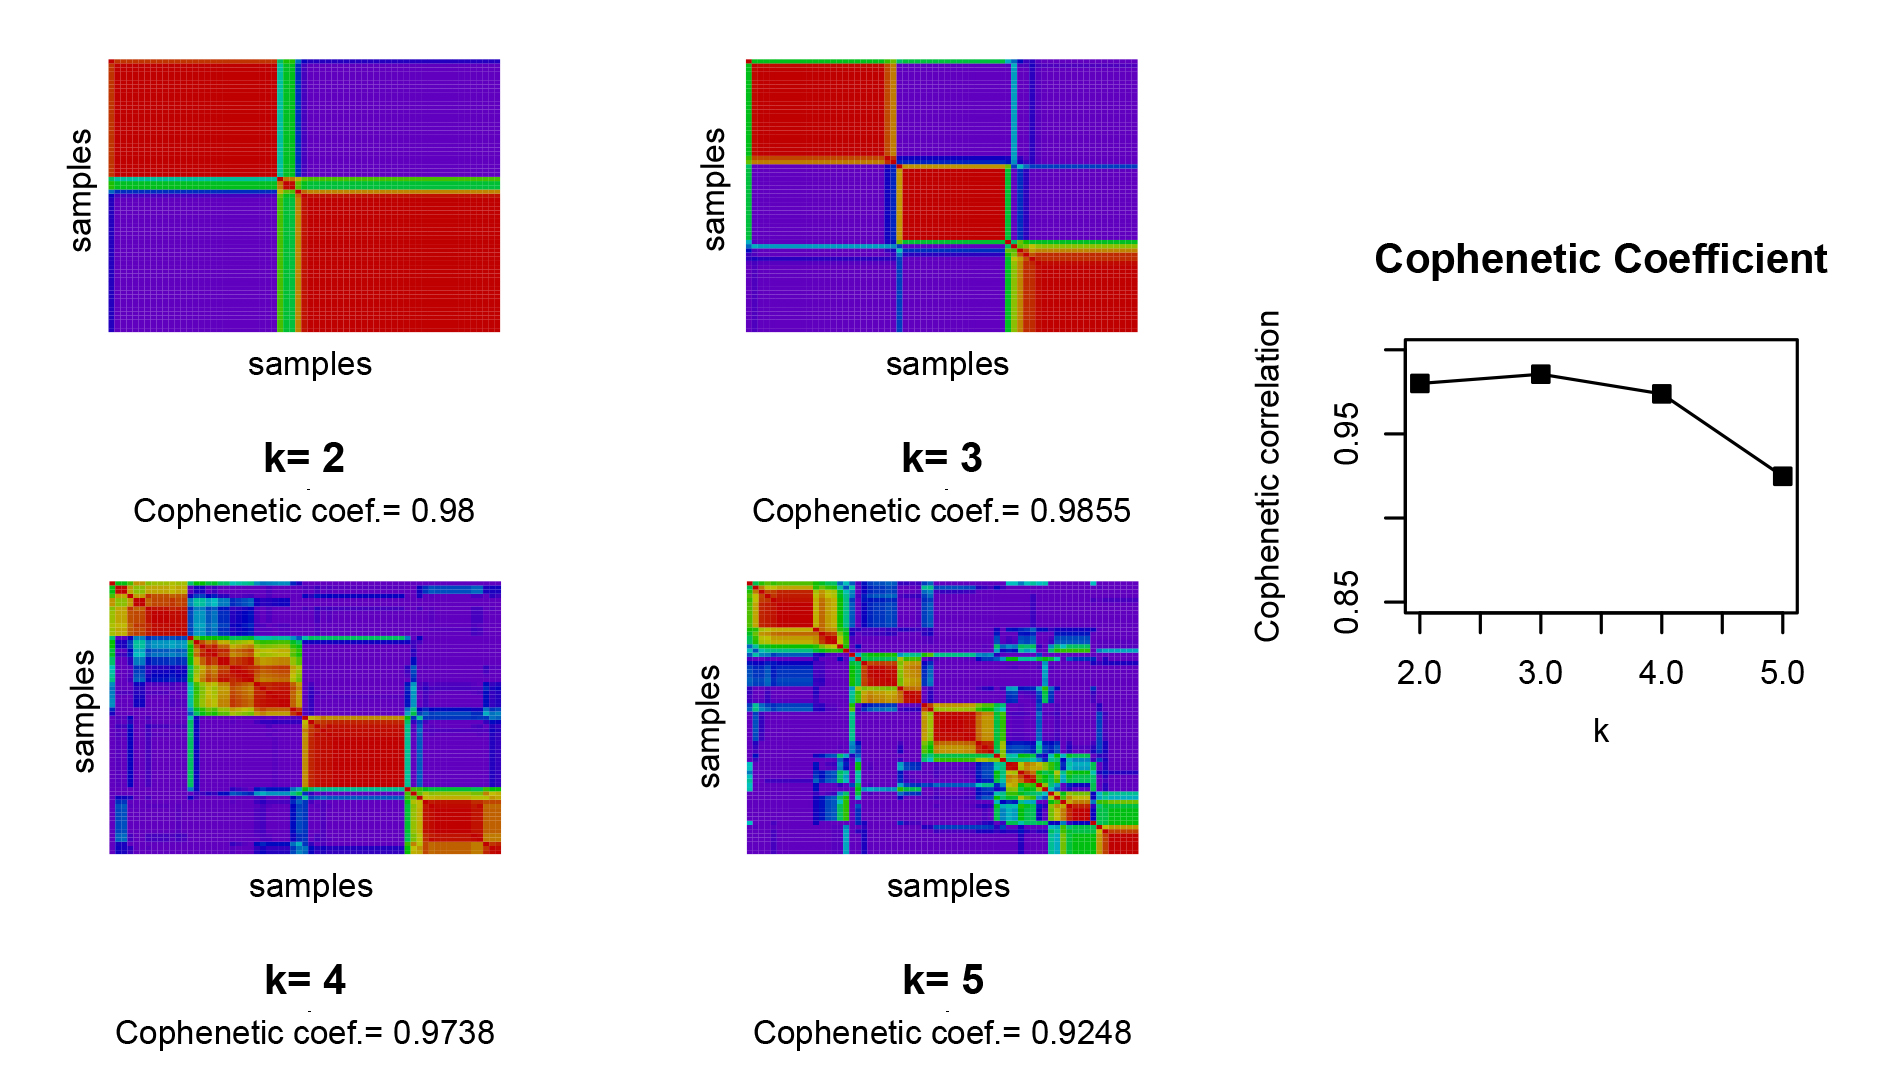
\includegraphics[width = 15cm]{Figures/consensus.jpg}}
\caption{Example of NMF results obtained for molecular subtype identification of Fus-AD-f dataset.}
\label{fig:consensus}
\end{figure}


\section{Molecular Subtype Identification} \label{subtype-method}

For the molecular subtype identification step, only those datasets which contained more than 30 case samples were eligible. This step was performed similarly to the selection of core samples. However, instead of using the complete dataset, the method was applied exclusively to the case samples of each dataset. The \verb|nmfconsensus| function was again leveraged with the same input parameters, except for the final $k$ value, which in this process took a value of 5, meaning that the best clustering could be between 2 and 5 groups. The best clustering is given by the $k$ with higher cophenetic coefficient, as seen in Fig. \ref{fig:consensus} where the best clustering is $k=3$. Then, the case samples were partitioned according to the membership list result.

\section{Cell Proportion Estimation} \label{cells-method}

\subsection{Immune cell types} \label{immune-method}

The immune cell types proportion was obtained through CIBERSORTx web services. First, the mixture file, which is the gene expression matrix, must be in tab-delimited tabular format with .txt extension and no missing entries. Also, the mixture file should be in non-log scale. Second, the user must have previously prepared the signature matrix; in this case, the LM22 signature matrix was employed \cite{newman15}. LM22 is a validated leukocyte gene signature matrix which includes 547 genes that can discriminate 22 human hematopoietic cells from bulk RNA-seq expression data; it comprises of seven T-cell types, plasma cells, memory and naïve B-cells, myeloid subsets, and natural killer cells (NK). After uploading both matrices to CIBERSORTx, the parameters for imputing cell fractions by a custom analysis were selected. To configure the input, the LM22 file must be chosen as the signature matrix and the gene expression file of interest as the mixture file. Then, B-mode of batch correction was selected since it is suggested to be used with bulk data, and the LM22 source GEP file (included in CIBERSORTx) was set for the optional source GEP file. Lastly, the quantile normalization was disabled (recommended for RNA-seq data) and the analysis was ran with 100 permutations (for significance) and in relative mode. This process was performed over each partitioned dataset and estimated molecular subtypes.

The resulting matrix contained the relative values of the 22 immune cell types within each sample. Therefore, in order to estimate a change between control and case (and case subtype), the mean of each immune cell type across the control and case samples were calculated. Afterwards, an unpaired $t$-test was implemented over the control and case mean of each cell type adjusted for FDR. The change was considered significant if the q-value was below 0.05, and the direction was defined by the difference in means of the cell type between control and case.

\subsection{Brain cell types} \label{brain-method}

On the other hand, the relative brain cell type proportion was resulted from \textit{BRETIGEA} R package. The \verb|brainCells| function was applied to each partitioned dataset and estimated molecular subtypes in log scale with 50 marker genes (suggested value from the authors) and specified for human. BRETIGEA includes the marker genes for six brain cell types (mentioned in Section \ref{cellprop}), so the same procedure done for immune cells was carried out, but only for six cell types. The steps are (i) calculate the mean for each cell across the control and case samples, and (ii) estimate the change with a $t$-test adjusted for FDR. Once again, the change was considered significant if the resulted q-value was less than 0.05.

\section{Differential Gene Expression Analysis} \label{dgea}

As mentioned in Section \ref{rna-seq}, the measures of the RNA-seq expression data can be given in different scales; in this study, the original databases were reported in number of reads, RPKM and FPKM. Hence, the resulting integrated databases were continuous data. The DGE analysis was performed with \textit{limma} package since it can manipulate this type of data. Nonetheless, before inputting the data into \textit{limma}'s functions, the datasets were transformed into logarithm based two scale with a pseudocount of 1 (to avoid logarithm of zero). Then, a design matrix was defined using \verb|model.matrix| function of the \textit{stat} package, which expands the factors to a set of dummy variables. The factors were control or case for each sample in the dataset, and the formula excluded the intercept.

Additionally, a contrast matrix was defined using \verb|makeContrast| function of \textit{limma}; the contrast matrix expresses the specified contrasts between the variables of the design matrix as a numeric matrix. Afterwards, the function \verb|lmFit| of \textit{limma}, which fits a linear model for each gene given a series of samples, was applied to the transformed data and the design matrix. Subsequently, the contrast matrix and the linear model are fed to \verb|contrasts.matrix| in order to estimate the coefficients and standard errors for the set of contrasts. Hence, this function adjusts the coefficients of the fitted model to the set of contrasts. Finally, the adjusted model is introduced to \verb|eBayes| function, without trend, to compute statistics (t-statistic, and F-statistic) and log-odds of differential expression using an empirical Bayes method which compresses the genewise-wise residual variances towards a common value or a global trend \cite{ebayes}. The resulted top-ranked genes were extracted with \verb|toptable|; the reported q-values are adjusted for multiple testing using Benjamini \& Hochberg since it controls the expected FDR, which was set to 0.05 in this study. Finally, the heatmaps were created with \textit{pheatmap} \cite{pheatmap} package and \verb|heatmap.2| function.

\section{Alternative Copy Number Variation} \label{cnv-method}

Copy number variation (CNV) refers to a DNA segment of one or more kilobases (kb) large that has a variable copy number when compared to a reference genome. Evidence has indicated that some CNVs have no apparent phenotype, while others have been definitively associated with diseases. Also, interactions with genetic or environmental factors might influence the detectability of a CNV phenotype \cite{clancy}. Therefore, the importance to identify possible CNV in the studied NDs.

The method for calculating the alternative CNV used in this work is similar to \cite{patel}. The first step to calculate the alternative CNV was to match the gene symbols of the expression matrix with their start and end position in the genome. The positions were obtained with a processed comprehensive gene annotation GTF file (GRCh38.p13) from GENCODE \cite{gencode}. When performing this match, a problem was caused by the many alias that the genes have. Hence, the \textit{limma} function, \verb|alias2SymbolTable|, was leveraged in order to solve this problem, however this function only recovered a few gene symbols. Then, the "NCBI gene information file" was downloaded; it contains the official gene symbols and the alias of the genes. The gene symbols of the expression matrix were related to the names of the genes in the GTF and the alias in the gene information file. In the end, the matching process was achieved with low number of unknown genes. Afterwards, the RNA segment (bypass for the DNA segment mentioned above) was defined with a 50 genes window. Therefore, the resulting matrix, named CNV matrix, had the samples as columns and filled with the expression mean of the 50 genes moving window; the row names were represented with the chromosome number, starting and ending gene.

Finally, the CNV plots were generated using \textit{karyploteR} \cite{karyoploter} and \textit{CopyNumberPlots} \cite{cnplots} R packages. Once again the heatmaps were created with \verb|heatmap.2| function of the \textit{pheatmap} package. To obtain the CNV plot, it was needed to calculate the mean of windows of ten segments (rows of the CNV matrix), which represented the gray lines on the graph. Additionally, the mean of log fold change (LFC) (obtained in Section \ref{dgea}) for the same segments of genes were used as the Copy Number (CN) value that appears in both heatmap and CNV plots. Moreover, the start and finish position of each segment had to be defined; then, some required information was extracted from the processed GTF in order to ultimately create the graphs.

\section{Functional Analysis} \label{path-method}

For the functional analysis, two methods were employed leveraging one main package. First, the Molecular Signature Database was retrieved with \verb|msifdbr| specifying for \textit{Homo sapiens} and the category C5. The C5 collection contains the GO resource (which includes biological process, cellular component, and molecular function ontologies) and the Human Phenotype Ontology, which in total has 14,765 gene sets. Moreover, for this analysis, only the gene set names and the human gene symbols were kept in a data frame; i.e. a term to gene data frame.

The next step consisted in generating the input data for ORA and GSEA. The former required a list of the DEG symbols in decreasing order of their LFC values. The latter needed a list of all gene symbols with their LFC in decreasing order. Finally, using \verb|enricher| and \verb|GSEA| functions of the \textit{clusterProfiler} package, the ORA and GSEA, respectively, were easily implemented. \verb|enricher| required the list created before along with the term to gene data frame; the remainder arguments were left as default. Likewise, \verb|GSEA| needed the list of all genes and the term to gene data frame as input, and the p-value cutoff was set to 0.05 for this study.

The visualizations were generated with \textit{enrichplot} package. Eight different graphs were able to be plotted using distinct functions and the resulting objects of the aforementioned analyses. In Table \ref{tab:plots}, the type of analysis is associated with the possible visualizations; the generated visualizations for this research project are marked with bold font.

\begin{table}[ht]
\centering
\caption{Functional analysis method and available visualization association.}
\label{tab:plots}
\begin{tabular}{lll}
\hline
\multicolumn{1}{c}{\textbf{Analysis}} & \multicolumn{1}{c}{\textbf{Visualization}} & \multicolumn{1}{c}{\textbf{Function}} \\ \hline
ORA         & \textbf{Bar plot}                                    & barplot   \\
GSEA        & \textbf{Running score and preranked list}            & gseaplot  \\
            & Ranked list of genes belong to the specific gene set & gsearank  \\
            & Ridgeline plot for expression distribution           & ridgeplot \\
ORA \& GSEA & \textbf{Gene-concept network}                        & cnetplot  \\
            & \textbf{Enrichment Map}                              & emapplot  \\
            & \textbf{Dot plot}                                    & dotplot   \\
            & \textbf{UpSet Plot}                                  & upsetplot \\
            & \textbf{Heatmap-like functional classification}      & heatplot  \\ \hline
\end{tabular}
\end{table}

\section{Drug Repurposing} \label{drug-method}

The drug repurposing analysis comprised of few lines of codes. \textit{PharmacoGx} and \textit{biomaRt} packages were leveraged for this process. At first, the gene symbols of the datasets were replaced with the Ensembl gene ID by the latter package since the former contains the gene set-drug relation in Ensembl language. After, a data frame was created using the Ensembl IDs and the direction of the LFC (positive or negative) calculated in Section \ref{dgea}. The CMAP perturbation dataset, an array of drug perturbation signatures, was retrieved by the \verb|downloadPertSig| function. Subsequently, the \verb|connectivityScore| was applied to the previously created data frame along with the perturbation dataset with FGSEA method and 100 permutations (for significance analysis). The result included the connectivity score and p-value; again the drug selection was considered significant if the p-value was lower than 0.05. Finally, this data frame was sorted by connectivity score in decreasing order and the first three or four drugs of the list were further investigated.

\section{GWAS Comparison} \label{gwas-method}

The last phase was the comparison of GWAS with the DEGs resulted from previous analyses. The followed process was guided by the lecture \cite{Prokob}. The GWAS Catalog database was downloaded from the official website, version GRCh38.p13 and dbSNP Build 153. Then, it was filtered by mapped trait, one of the NDs of interest at a time (i.e. "Alzheimer's disease", "Parkinson's disease", and "Huntington's disease: disease progression measurement"), and variants with p-value less than 0.001. Afterwards, the SNPs were split into common and rare variants according to the risk allele frequency (RAF): variants with RAF less than 5\% were set as rare. Its important to mentioned that variants for HD were not split.

The rare SNPs IDs, and all the HD SNPs IDs, were introduced into the proxy search of SNiPA in order to find possible LD variants. These variants were searched in the genome assembly GRCh37, genome annotation Ensembl 87 and variant set of 1,000 Genomes Phase 3 version 5 in European population with a threshold for the minimum correlation coefficient between sentinels and proxies of 0.8. The resulting list of proxy variants was downloaded, variants which are not annotated in GWAS Catalog. The following steps were applied to rare, common and unnanotated variants. In order to identify possible impacts on the structure and function of coding proteins, the list of variants was input to PolyPhen-2 with genome assembly GRCh37/hg19. PolyPhen-2 outputs a tab-delimited file with the possible affected proteins (in UniProt ID) and impact of each variant. Finally, the SNPs which did not have an impact on proteins were fed to RegulomeDB web service. As mentioned in Section \ref{gwas}, RegulomeDB outputs a score for each variant which represents the variant's relevance; the resulting variants with a score higher or equal than $3a$ were kept for the last comparison. Finally, the genes which were affected by the investigated variants were compared to the genes obtained in Section \ref{dgea}.